\chapter{Grundlagen}

\section{2-Dimensionales Punktediagramm}
Das 2-Dimensionale Punktediagramm ist der am meisten verwendete Typ des Punktediagramms.

\subsection{Interpolation}
Für eine verbesserte Ansicht des Punktediagramms fügt man oft eine Linie ein, die alle im Punktediagramm vorhandenen Punkte verbindet. Sie stellt den Verlauf des Wertes zwischen den Datenpunkten dar.

Die unkomplizierteste, am meisten Verwendete Interpolation ist die \textbf{lineare Interpolation} (Abbildung \ref{fig:linear}). Zwei nebeneinanderliegende Punkte werden durch einer Gerade verbunden.

\begin{figure}[htbp]
	\centering
	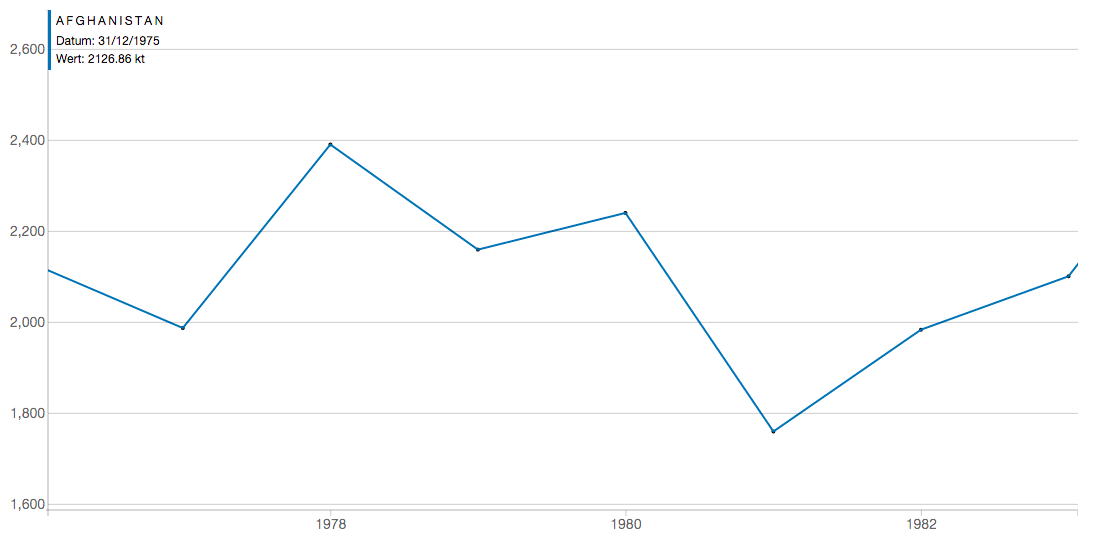
\includegraphics[width=0.80\linewidth]{images/linear}
	\caption[Lineare Interpolation]{Beispiel der linearen Interpolation am Datensatz des CO2-Verbrauchs von Afghanistan.}
	\label{fig:linear}
\end{figure}

Die Interpolation mit Splines, der \textbf{Kubisch Hermitescher Spline} (Abbildung \ref{fig:cardinal}).

\begin{figure}[htbp]
	\centering
	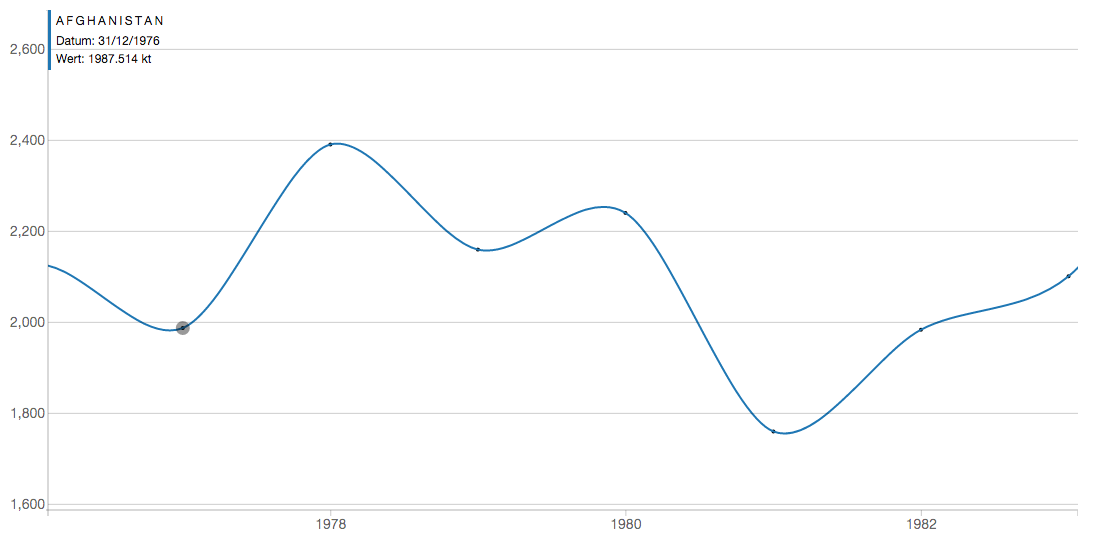
\includegraphics[width=0.80\linewidth]{images/cardinal}
	\caption[Kubischer Hermitescher Spline]{Beispiel des Kubischen Hermetischen Spline am Datensatz des CO2-Verbrauchs von Afghanistan.}
	\label{fig:cardinal}
\end{figure}

\subsection{Linien}
\subsection{Tooltip}
\subsection{Anzeige von mehreren Datensätzen}

\section{3-Dimensionaler Punktediagramm}

\subsection{Kamera}
\subsection{Projektion}
\subsection{Orthographische und Perspektivische Kamera}
\subsection{Transition zwischen Projektionen}

\section{n-Dimensionaler Punktediagramm}